\documentclass[a4paper]{article}
\usepackage[utf8]{inputenc}
\usepackage[italian]{babel}
\usepackage{import}
\usepackage{graphicx}
\usepackage{float}
\usepackage[margin=1.2in]{geometry}
\usepackage[12pt]{extsizes}
\usepackage{color}
\usepackage{listings}
\usepackage[bottom,flushmargin,hang,multiple]{footmisc}
\usepackage{titlesec}
\usepackage{url}
\usepackage{upquote}
\usepackage{csquotes}
\usepackage{biblatex}
\definecolor{purple}{RGB}{91, 72, 181}
\definecolor{darkviolet}{rgb}{0.58, 0.0, 0.83}
\definecolor{royalblue}{RGB}{242, 73, 214}
\definecolor{orange}{RGB}{227, 72, 41}
\definecolor{lightgreen}{RGB}{164, 194, 14}

\definecolor{mediumgray}{rgb}{0.3, 0.4, 0.4}
\definecolor{forestgreen}{rgb}{0.13, 0.55, 0.13}
\definecolor{crimson}{rgb}{0.86, 0.8, 0.24}

\addbibresource{./bibliografia/bibliografia.bib}

\linespread{1.5}

\graphicspath{ {./images/} }

\setcounter{secnumdepth}{4}
\setcounter{tocdepth}{4}

\titleformat{\paragraph}{\normalfont\normalsize\bfseries}{\theparagraph}{1em}{}
\titlespacing*{\paragraph}{0pt}{3.25ex plus 1ex minus .2ex}{1.5ex plus .2ex}

\lstset{aboveskip=30pt,belowskip=30pt}

\lstdefinestyle{JSES6Base}{
  backgroundcolor=\color{white},
  basicstyle=\ttfamily,
  breakatwhitespace=false,
  breaklines=false,
  captionpos=b,
  columns=fullflexible,
  commentstyle=\color{mediumgray}\upshape,
  emph={},
  emphstyle=\color{crimson},
  extendedchars=true,  % requires inputenc
  fontadjust=true,
  frame=single,
  identifierstyle=\color{black},
  keepspaces=true,
  keywordstyle=\color{purple},
  keywordstyle={[2]\color{darkviolet}},
  keywordstyle={[3]\color{royalblue}},
  keywordstyle={[4]\color{orange}},
  keywordstyle={[5]\color{lightgreen}},
  numbers=left,
  numbersep=5pt,
  numberstyle=\tiny\color{black},
  rulecolor=\color{black},
  showlines=true,
  showspaces=false,
  showstringspaces=false,
  showtabs=false,
  stringstyle=\color{forestgreen},
  tabsize=2,
  title=\lstname,
  upquote=true  % requires textcomp
}

\lstdefinestyle{JavaScript}{
  language=JavaScript,
  style=JSES6Base
}

\lstdefinestyle{ES6}{
  language=ES6,
  style=JSES6Base
}

\lstdefinelanguage{JavaScript}{
  morekeywords=[1]{break, continue, delete, else, for, function, if, in,
    new, return, this, typeof, var, void, while, with, render, getElementById, width, height, contract, address, event, uint256, public, returns, emit, pragma, describe, it},
  % Literals, primitive types, and reference types.
  morekeywords=[2]{false, null, true, boolean, number, undefined,
    Array, Boolean, Date, Math, Number, String, Object, onClick, Map, onChange},
  morekeywords=[3]{h1, div, p, button, TextField},
  morekeywords=[4]{React, ., Component, Saluto, Convenevoli, Contatore, setContatore, useState, contatore,
    Button, ContatoreConTitolo, handleSearch, searchInput, target, value, setActiveCoinsList, coinsList, coinName, coinSymbol, coin,
    coinsToSellAmounts, setCoinsToSellAmounts, coinsToAcceptAmounts, setCoinsToAcceptAmounts, setCoinsList, activeCoinsList,
    activeStep, setActiveStep, web3Instance, userAccount, fetchCoins, setLoadingCoinList, newCoinsList, Contratto},
  morekeywords=[5]{},
  sensitive,
  morecomment=[s]{/*}{*/},
  morecomment=[l]//,
  morecomment=[s]{/**}{*/}, % JavaDoc style comments
  morestring=[b]',
  morestring=[b]"
}[keywords, comments, strings]

\lstalias[]{ES6}[ECMAScript2015]{JavaScript}

\lstdefinelanguage[ECMAScript2015]{JavaScript}[]{JavaScript}{
  morekeywords=[1]{await, async, case, catch, class, const, default, do,
    enum, export, extends, finally, from, implements, import, instanceof,
    let, static, super, switch, throw, try},
  morestring=[b]` % Interpolation strings.
}


\title{Progettazione e realizzazione di un exchange decentralizzato per lo scambio di token ERC20 per la piattaforma CommonsHood}

\begin{document}
    \tableofcontents
    \newpage
    \section{Background}
    \subsection{CommonsHood}
    CommonsHood è un’applicazione web basata su smart contract per blockchain Ethereum che ha lo scopo di fornire alla comunità strumenti per l’inclusione finanziaria e per supportare l’economia locale delle comunità di cittadini.
    Gli utenti, una volta registrati sulla piattaforma, possono creare monete, ossia token crittografici Ethereum basati sullo standard ERC-20, questi possono rappresentare beni di valore o servizi.
    Un altro asset che gli utenti possono creare e possedere sono i coupon, questi sono rappresentati da token non fungibili basati sullo standard ERC-721, in questo modo ogni singolo coupon è univoco e diverso dagli altri.
    Gli utenti possono utilizzare i coupon per ottenere prestazioni e servizi.
    \newline
    Un'altra funzionalità offerta dall'applicazione è la possibilità di creare crowdsales, questi sono usati per ottenere fondi per finanziare progetti o eventi, dando, in cambio, ai finanziatori monete oppure coupons.
    Un esempio di un'interazione con la piattaforma potrebbe essere: il negozio di attrezzature da sub \emph{"Sotto il Mar"} crea un account su CommonsHood. Crea, inoltre, una moneta chiamata \emph{"Doblone"}, questa può essere spesa in negozio
    per acquistare le attrezzature. Oltre alla vendita, il negozio noleggia anche le attrezzature, perciò crea dei coupon che possono essere utilizzati per ottenere i prodotti a noleggio.
    Inoltre, una stanza ha bisogno di ristrutturazioni perciò viene creata una crowdsale per ottenere il finanziamento necessario, in cambio vengono offerti dei coupon del negozio.
    
    \subsection{Blockchain}
    Una blockchain è un registro aperto e distribuito di dati, strutturato come una catena di blocchi contenenti le transazioni.
    Le transazioni solitamente rappresentano uno scambio di monete, chiamate token. Ogni blockchain ha un token proprio.
    I dati risiedono su unità computazionali chiamati \emph{nodi}, questi, come mostrato nell'immagine \ref{fig:node},
    sono interconnessi e comunicano tra loro per mantenere i dati di tutti i nodi aggiornati\cite{nodo}.
    Un account su una blockchain è costituito da una coppia di chiavi:
    \begin{itemize}
      \item pubblico: è un indirizzo sulla blockchain, i token nella rete sono registrati come appartenenti ad un indirizzo;
      \item privato: è come una password che l'utente utilizza per accedere ai propri fondi.
    \end{itemize}
    \begin{figure}[ht]
      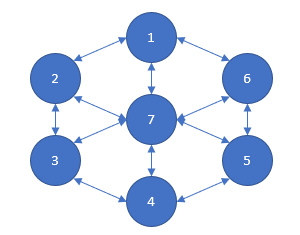
\includegraphics[scale=0.8]{node.png}
      \centering
      \caption{Rete di nodi}
      \centering
      \label{fig:node}
    \end{figure}
    \subsubsection{I nodi}
    Le responsabilità di un nodo sono principalmente:
    \begin{itemize}
      \item Controllo della validità di un nuovo record di dati, chiamato anche transazione, e accettarlo o rifiutarlo;
      \item Nel caso di un record valido, salvataggio della transazione nel registro locale del nodo;
      \item Comunicazione e distribuzione della transazione agli altri nodi. In questo modo tutti i nodi hanno la stessa versione del registro.
    \end{itemize}
    \subsubsection{Le caratteristiche di una blockchain}
    Le caratteristiche principali della tecnologia blockchain sono:
    \begin{itemize}
      \item Decentralizzazione: le informazioni contenute nel registro digitale vengono distribuite tra più nodi, così da garantire sicurezza e resilienza dei sistemi anche in caso di attacco a uno dei nodi o in caso di perdita di un nodo.
      \item Tracciabilità: ogni elemento salvato nel registro è tracciabile in ogni sua parte e se ne può risalire all’esatta provenienza e alle eventuali modifiche apportate nel corso del tempo, con una precisione assoluta.
      \item Disintermediazione: i singoli nodi della blockchain certificano le informazioni distribuite, rendendo quindi del tutto inutile la presenza di enti centrali o di aziende per la certificazione dei dati.
      \item Trasparenza: il contenuto del registro è visibile a tutti ed è facilmente consultabile e verificabile da ogni nodo della rete ma anche tramite servizi che interrogano la blockchain senza apportare modifiche. Nessuno può nascondere o modificare dati senza che l'intera rete venga a saperlo.
      \item Solidità del registro: dopo aver aggiunto un'informazione al registro, essa non può essere modificata senza il consenso di tutta la rete.
      \item Programmabilità: le operazioni di transazione possono anche essere programmate nel tempo, così da poter attendere il verificarsi di determinate condizioni prima di procedere con l'inserimento o la modifica\cite{blockchain1}.
    \end{itemize}
    \subsubsection{Smart contracts}
    Le blockchain permettono d'implementare codici e funzioni all'interno di esse, questi sono chiamati smart contracts e permettono l'esecuzione di operazioni quando predeterminate condizioni si avverano.
    Sono tipicamente usate per automatizzare l'esecuzione di un accordo, in questo modo tutti i partecipanti possono verificarne immediatamente i risultati, senza aver bisogno di un intermediario.
    Possono, inoltre, essere utilizzate per automatizzare workflow, innescando azioni successive al raggiungimento di certe condizioni\cite{smartcontracts}.
    
    \subsection{Ethereum}
    Ethereum è una piattaforma blockchain decentralizzata che stabilisce una rete peer-to-peer che esegue e verifica smart contracts in modo sicuro.
    Gli smart contracts permettono transazioni tra gli utenti senza la necessità di un autorità centrale.
    Le transazioni sono immutabili, verificabili, e distribuiti in modo sicuro sulla rete. Le transazioni sono inviate e ricevute da account Ethereum creati dagli utenti.
    Come costo per il processamento di una transazione sulla rete, l'utente deve spendere Ether (ETH), la criptovaluta nativa di Ethereum\cite{ethereum}.
    \subsubsection{Token Ethereum}
    Ethereum permette la creazione di token crittografici all'interno della sua rete. Questi token non sono altro che smart contracts scritti seguendo specificazioni stabilite
    dagli sviluppatori della rete. I token possono essere di tipi di differenti, a seconda delle specificazioni seguite. In Ethereum ci sono principalmente due tipi di token: token ERC-20 e NFT.
    \paragraph{Token ERC-20}
    I token ERC-20 sono il tipo di token più diffuso sulla rete Ethereum, sono lo standard per la definizione di token fungibili\cite{erc20}, ossia i singoli token sono indistinguibili e intercambiabili tra loro.
    Un token ERC-20 implementa le specificazioni indicate nell'EIP-20 che richiede nello smart contract del token la presenza di diversi metodi. I più importanti metodi richiesti sono:
    \begin{itemize}
      \item \verb|balanceOf(address _owner)|: restituisce la quantità di token posseduto da \verb|_owner|;
      \item \verb|transfer(address _to, uint256 _value)|: trasferisce una quantità di token indicata da \verb|_value| all'indirizzo \verb|_to|;
      \item \verb|transferFrom(address _from, address _to, uint256 _value)|: trasferisce una quantità \verb|_value| di token dall'indirizzo \verb|_from| all'indirizzo \verb|_to|;
      \item \verb|approve(address _spender, uint256 _value)|: permette all'indirizzo \verb|_spender| di ritirare fino a \verb|_value| token dall'account\cite{eip20}.
    \end{itemize}
    \paragraph{NFT}
    I Non Fungible Tokens sono, appunto, token non fungibili, ossia ogni token è univoco e non intercambiabile con un altro. Sono utilizzati per replicare le proprietà tipiche
    di un oggetto fisico come la scarsità, l'unicità e la possibilità di dimostrare la proprietà del token\cite{nft}.
    Data la natura del token, l'uso più comune di questi token è la creazione di arte digitale\cite{nftuse}.
    \newline
    Gli NFT seguono lo standard dettato dall'EIP-721.
    \subsubsection{Smart contracts in Ethereum}
    In Ethereum gli smart contracts sono considerati come account, questo significa che hanno un saldo e possono inviare transazioni sulla rete. A differenza di un normale account, però,
    gli smart contracts non sono controllati dagli utenti ma eseguono il codice con cui sono stati programmati. Gli account user possono interagire con uno smart contract inviando una transazione
    che effettua una chiamata a una funzione definita nello smart contract. Di default questi contratti non possono essere eliminati e le interazioni con essi sono irreversibili.
    \newline
    Il codice di uno smart contract si scrive utilizzando \emph{Solidity}, un linguaggio object-oriented usato per implementare smart contracts su diverse piattaforme blockchain.
    Di seguito un esempio di uno smart contract semplice:
    \begin{lstlisting}[style=ES6, title={Esempio codice di uno smart contract}]
      pragma solidity ^0.5.2;

      contract EsempioContratto() {
        address public owner;
        
        event EsempioEvento(
          uint256 parametroEvento
        )

        function esempioFunzione(
          uint256 _parametro
        ) public returns (uint256) {
          emit EsempioEvento(_parametro)
          return _parametro
        }
      }\end{lstlisting}
      Solitamente uno smart contract inizia con la dichiarazione della versione di solidity usata per la scrittura del codice, in questo modo il compilatore, se di versione superiore, rifiuta la compilazione del codice.
      Per far questo si scrive: \newline \verb|pragma solidity [versione]|. Nell'esempio precedente la versione è dichiarata nella prima riga, in questo caso la versione indicata è superiore a 0.5.2.
      \newline
      Una volta dichiarata la versione, inizia il codice dello smart contract, questo viene indicato con \verb|contract [nome contratto]()|. Prendendo sempre come riferimento l'esempio precedente,
      alla riga 4 viene dichiarata una variabile chiamata owner con visibilità \verb|public| e tipo \verb|address|, ossia un indirizzo Ethereum. Ci sono 4 livelli di visibilità per le variabili e le funzioni:
      \begin{itemize}
        \item \verb|public|: le funzioni possono essere chiamate anche da contratti esterni, per le variabili vengono generate in automatico delle funzioni getter implicite;
        \item \verb|external|: le funzioni e le variabili possono essere accedute solo dall'esterno e non internamente nel contratto;
        \item \verb|internal|: le funzioni e le variabili possono essere accedute dentro il contratto stesso e i contratti derivati;
        \item \verb|private|: visibili solo nel contratto in cui le variabili e le funzioni sono definite\cite{solidityvisibility}.
      \end{itemize}
      Solidity fornisce numerosi tipi per le variabili, di cui quelle usate in questa tesi sono:
      \begin{itemize}
        \item \verb|bool|: per indicare una variabile booleana;
        \item \verb|uint|: per indicare un intero senza segno, può avere diverse dimensioni aggiungendo il numero di bits, ad esempio \verb|uint256|;
        \item \verb|address|: per indicare un indirizzo Ethereum;
        \item \verb|mapping|: per indicare un dizionario con chiavi di ricerca e valori associati\cite{soliditytypes}.
      \end{itemize}
      Alla riga 6 è stato dichiarato un evento, ossia uno strumento utile per fare logging delle transazioni e per permettere agli utenti di mettersi in ascolto di questi eventi.
      Un evento può contenere dati aggiuntivi, in questo caso l'evento \verb|EsempioEvento| contiene il dato \verb|parametroEvento| di tipo uin256.
      Per emettere un evento si utilizza \verb|emit [nome evento](dati evento)|, come mostrato alla riga 13.
      \newline
      Alla riga 10 è stata dichiarata una funzione di nome \verb|esempioFunzione|, con visibilità \verb|public|, con parametro \verb|_parametro| e che restituisce un valore di tipo \verb|uin256|.
      Questa funzione esegue solo due operazioni: emette l'evento \verb|EsempioEvento| e restituisce un valore. 

    \subsection{OpenZeppelin}
    OpenZeppelin è una libreria per lo sviluppo di smart contracts sicuri. Le principali funzionalità fornite da OpenZeppelin sono:
    \begin{itemize}
    \item Implementazione dei diversi standard dei token Ethereum;
    \item Gestione del controllo degli accessi agli smart contracts;
    \item Componenti Solidity riutilizzabili per creare smart contracts\cite{openzeppelin}.
    \end{itemize}

    \subsection{Metamask}
    Metamask è un'estensione del web browser. Questo software permette di connettere il browser con
    applicazioni decentralizzate basate sulla piattaforma Ethereum. Metamask permette la gestione di
    wallet Ethereum, la ricezione e l'invio di criptomonete basate su Ethereum, e l'interazione con
    applicazioni decentralizzate. L'estensione, inoltre, fornisce le API Ethereum web3, in questo
    modo le applicazioni sono in grado di leggere dati sulla blockchain\cite{metamask}.

    \subsection{ReactJS}
    React è una libreria JavaScript open-source per lo sviluppo d'interfacce utente.
    \subsubsection{Caratteristiche di ReactJS}
    React fornisce numerosi strumenti che facilitano lo sviluppo di un'interfaccia grafica. Di seguito sono descritti quelli utilizzati in questa tesi.
    \paragraph{Componenti}
    I Componenti permettono di suddividere la UI in parti indipendenti, riutilizzabili e di pensare a ognuna di esse in modo isolato.
    Per definire un componente è necessario implementare una funzione JavaScript, ad esempio:

    \begin{lstlisting}[style=ES6, title={Esempio componente}]
        function Saluto(props) {
            return <h1>Ciao, {props.nome}</h1>;
        }\end{lstlisting}

    Questo componente accetta un oggetto parametro contenente dati sotto forma di una singola
    "props", il quale è un oggetto parametro avente dati al suo interno.
    Per renderizzare un componente bisogna utilizzare la funzione \verb|ReactDOM.render()|,
    passandole come parametri il componente da visualizzare e il riferimento al componente padre.
    Se si volesse, quindi, renderizzare il componente \verb|Saluto|, passando "\emph{Martina}" come parametro \verb|nome|, il codice potrebbe essere:
    
    \begin{lstlisting}[style=ES6, title={Esempio composizione di componenti}]
      ReactDOM.render(
        <Saluto nome="Martina"/>, 
        document.getElementById('root')
      );\end{lstlisting}
    
    I componenti, inoltre, possono essere composte da altri componenti. In questo caso,
    renderizzando il componente padre, verranno visualizzati anche i componenti figli. Ad esempio, 
    si potrebbe avere un componente \verb|Convenevoli| che contiene multipli componenti \verb|Saluto|:
    \begin{lstlisting}[style=ES6, title={Esempio renderizzazione componente}]
      function Convenevoli() {
        return (
          <div>
            <Saluto nome="Sara" />
            <Saluto nome="Cahal" />
            <Saluto nome="Edite" />
          </div>
        );
      }\end{lstlisting}

      \paragraph{Hook state}
      Un componente React di default è stateless. Usando la funzione \verb|useState()| si può
      aggiungere uno stato interno a un componente, React preserverà questo stato tra le ri-renderizzazioni.
      \verb|useState| ritorna una coppia: il valore dello stato corrente e una funzione che ci permette di aggiornarlo.
      La funzione ha un unico parametro ed è il suo stato iniziale. Ad esempio, se si volesse realizzare un contatore con un bottone che, alla sua pressione,
      aumenti il valore del contatore, si potrebbe scrivere il seguente codice:
      \begin{lstlisting}[style=ES6, title={Esempio contatore con stato interno}]
        function Contatore() {
          const [contatore, setContatore] = useState(0);
          return (
            <div>
              <p>Hai cliccato {contatore} volte</p>
              <button 
                onClick={() => setContatore(contatore + 1)}>
                Cliccami
              </button>
            </div>
          );
        }\end{lstlisting}

      \paragraph{Hook effect}
      Il costrutto \verb|useEffect()| permette l'esecuzione di funzioni a ogni renderizzazione da parte di React.
      Questa funzione viene utilizzata per effettuare operazioni nei vari stati del ciclo di vita di un componente.
      \newline
      Nel seguente esempio il titolo del documento viene aggiornato all'aumentare del valore del contatore, infatti, 
      a ogni aggiornamento del DOM da parte di React, viene chiamata la funzione passata a \verb|useEffect()|.
      \begin{lstlisting}[style=ES6, title={Esempio uso di useEffect()}]
        function ContatoreConTitolo() {
          const [contatore, setContatore] = useState(0);

          useEffect(() => {
            document.title = `Hai cliccato ${contatore} volte`;
          });

          return (
            <div>
              <p>Hai cliccato {contatore} volte</p>
              <button
                onClick={() => setContatore(contatore + 1)}>
                Cliccami
              </button>
            </div>
          );
        }\end{lstlisting}

        \subsection{Material-UI}
        Material-UI è una libreria per ReactJS per creare interfacce utente.
        La libreria contiene al suo interno numerosi componenti grafici,
        questi sono forniti di un tema di default, per modificare l'aspetto di
        un componente si può utilizzare la sua proprietà \verb|className|.
        \newline
        Nell'esempio seguente, preso da \cite{materialui}, vengono modificati le dimensione di un componente \verb|<Button>|:
        \begin{lstlisting}[style=ES6, title={Esempio modifica aspetto di un componente}]
          .Button {
            width: "100px",
            height: "100px"
          }

          <Button className="Button">\end{lstlisting}

        \subsection{Truffle e Ganache}
        Truffle e Ganache sono entrambi strumenti contenuti all'interno della suite software Truffle.
        Ganache permette la creazione di una blockchain Ethereum che viene eseguita in locale, semplificando, così,
        il deploy e il test degli smart contracts. Truffle è un software che facilita lo sviluppo di smart contracts.
        \newline
        I principali comandi di truffle utilizzati sono stati:
        \begin{itemize}
          \item \verb|truffle compile|, per compilare gli smart contracts;
          \item \verb|truffle test|, per eseguire i file di test;
          \item \verb|truffle deploy|\footnote{oppure truffle migrate}, per eseguire il deploy degli smart contracts\cite{truffle}.
        \end{itemize}
        \subsubsection{Creazione di un progetto Truffle}
        Per creare un progetto con Truffle si utilizza il comando \verb|truffle init| all'interno della sua cartella. Questo genera la struttura del progetto composta da quattro elementi:
        \begin{itemize}
          \item \verb|contracts/|: la cartella che conterrà gli smart contracts;
          \item \verb|migrations/|: la cartella che conterrà gli scripts per il deploy dei contratti;
          \item \verb|test/|: la cartella che conterrà i file per eseguire i test sui contratti;
          \item \verb|truffle-config.js|: il file di configurazione di Truffle.
        \end{itemize}
        \subsubsection{Compilazione degli smart contracts}
        Lanciando il comando \verb|truffle compile| nel progetto vengono compilati tutti gli smart contracts, ossia tutti file con estensione \verb|.sol|, presenti all'interno della cartella \verb|contracts/|.
        Questa operazione genera una nuova directory \verb|build/contracts| contenente un file \verb|.json| per ogni smart contract compilato. Questi file servono per il corretto funzionamento di Truffle quindi la modifica di essi è sconsigliata.
        Inoltre, contengono le ABI\footnote{Application Binary Interface} degli smart contracts, ossia delle interfacce che stanno tra un programma utente e la blockchain Ethereum. Queste sono necessarie perché gli smart contracts deployati sono sotto forma
        di codici binari e i loro dati sarebbero difficilmente comprensibili. Un' ABI, quindi, descrive le funzioni del suo smart contract ed interpreta i dati di questi metodi. Le  ABI saranno, perciò, necessarie durante l'implementazione dell'applicazione utente.
        \subsubsection{Deploy degli smart contracts}
        Il file \verb|truffle-config.js| permette di definire reti Ethereum che possono essere usate per eseguire il deploy degli smart contracts. Il file ha al suo interno un oggetto \verb|newtorks|, questo contiene la lista delle reti scritte nel seguente formato:
        \begin{lstlisting}[style=ES6, title={Esempio di definizione di una rete Ethereum}]
          <nome_rete>: {
            host: <host>,
            port: <port>,
            network_id: <network_id>
          }\end{lstlisting}
        Dove \verb|host| e \verb|port| indicano l'indirizzo e la porta della rete. \verb|network_id| è, invece, l'identificativo della rete.
        \newline
        Per fare il deploy su una rete specifica si aggiunge l'opzione \verb|--network| al comando \verb|truffle deploy|, perciò, ad esempio,
        se si volesse fare il deploy degli smart contracts su una rete Ethereum chiamata \verb|main|, il comando completo sarebbe:
        \begin{lstlisting}[style=ES6, title={Esempio di deploy specificando la rete}]
          truffle deploy --network main\end{lstlisting}
        Quest'opzione di specificare la rete di destinazione del deploy è utile perché è possibile effettuare il deploy non sulla rete principale di Ethereum, dove sarebbe presente una tassa di ETH, ma su una rete di test locale. 
        \subsubsection{Test degli smart contracts}
        Il comando \verb|truffle test| esegue tutti i file di test inclusi nella cartella \verb|test/|. Per eseguire, invece, un solo file di test lo si specifica nel comando. Quindi ad esempio: \verb|truffle test ./percorso/del/test/file.js|.
        I file di test sono tutti file presenti nella cartella \verb|test/| con una delle seguenti estensioni: \verb|.js|, \verb|.ts|, \verb|.es6|, \verb|.jsx| e \verb|.sol|.
        \newline
        Truffle si avvale di due framework per la scrittura di file di test: \emph{Mocha} e \emph{Chain}\cite{truffleframeworks}. Il primo è un framework per l'esecuzione di test su file Javascript. Il secondo è una libreria per la scrittura di asserzioni,
        ossia espressioni che indicano i valori attesi alla fine di un test.
        \newline
        Un tipico file di test ha la seguente forma:
        \begin{lstlisting}[style=ES6, title={Esempio di file di test}]
          const Contratto = artifacts.require(
            "<smart_contract_da_testare>");
          contract("Contratto", async accounts => {
            describe("<Funzionalita_da_testare>", async () => {
              it("<Comportamento_da_testare>", async () => {
                assert.equal(
                  <valore_ottenuto>,
                  <valore_atteso>,
                  "<messaggio_da_stampare>"
                );
              });
              it(
                ....
              )
            })
          })\end{lstlisting}
        La riga 1 serve per indicare un file di smart contract usato all'interno del test, per far questo si utilizza \verb|artifacts.require()|.
        

        \section{Scrittura e test dei smart contracts}
        \newpage

        \section{Implementazione dell'interfaccia grafica}
        L'interfaccia utente che implementa le funzionalità di scambio di token è stata divisa in due pagine.
        La prima è chiamata \emph{Create Sale} e, scegliendo i token da vendere e quelli da accettare, permette
        la creazione di una vendita. La seconda è chiamata \emph{Sales List} e permette di visualizzare la lista di tutte le vendite, sia quelle in corso
        che quelle terminate.
        \subsection{Create Sale}
        Il processo di creazione di una vendita è diviso in tre step.
        \begin{itemize}
          \item Nel primo step l'utente sceglie i token in suo possesso da mettere in vendita;
          \item Nel secondo step l'utente sceglie i token che accetta come pagamento per la vendita dei token scelti nel primo step;
          \item Nel terzo step viene mostrato all'utente un riassunto delle scelte fatte nei due step precedenti. In questo passo, inoltre, l'utente può
                impostare una data di scadenza della vendita.
        \end{itemize}
        In tutti e tre gli step sono presenti alcuni componenti grafici comuni, questi sono visibili nell'immagine \ref{fig:commonComponents}.
        \begin{figure}[H]
          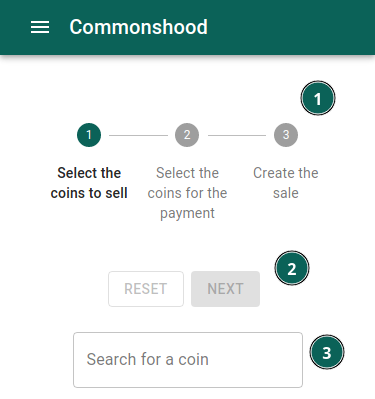
\includegraphics[width=\textwidth]{commonComponents.png}
          \caption{Componenti comuni}
          \centering
          \label{fig:commonComponents}
        \end{figure}
        Per mostrare graficamente il progresso nei diversi step è presente, in cima alla pagina, un componente
        \verb|<stepper>|, questo, come mostrato nell'immagine \ref{fig:commonComponents} al punto 1, indica all'utente gli step terminati e quelli ancora da completare.
        \newline
        Al di sotto, al punto 2, sono presenti due pulsanti per la navigazione nei vari step. Il primo permette di tornare allo step 1 azzerando tutti i parametri inseriti.
        Il secondo serve per avanzare allo step successivo.
        \newline
        Al punto 3 è presente un campo di inserimento per cercare una moneta in particolare.
        \subsubsection{Caricamento della pagina}
        Al caricamento della pagina vengono inizializzate alcune variabili, tra cui le più significative sono le seguenti:
        \begin{lstlisting}[style=ES6, title={Inizializzazione delle variabili al caricamento della pagina Create Sale}]
        const {web3Instance, userAccount} = props;
        const [coinsToSellAmounts,
               setCoinsToSellAmounts] = useState(new Map());
        const [coinsToAcceptAmounts,
               setCoinsToAcceptAmounts] = useState(new Map());
        const [coinsList, setCoinsList] = useState([]);
        const [activeCoinsList,
               setActiveCoinsList] = useState([]);
        const [activeStep, setActiveStep] = useState(0);\end{lstlisting}
        \verb|web3Instance| contiene l'istanza di web3 mentre \verb|userAccount| contiene l'indirizzo Ethereum dell'utente corrente, questi vengono passati alla pagina come props.
        \newline
        \verb|coinsToSellAmounts| e \verb|coinsToAcceptAmounts| sono variabili dotate di stato ed entrambi sono di tipo \verb|Map|, ossia un dizionario con chiavi di ricerca e valori associati.
        Vengono usate per mantenere le quantità delle monete scelte da mettere in vendita, per la prima variabile, oppure quelle da accettare come pagamento, nel caso della seconda variabile.
        Hanno come chiavi di ricerca le monete mentre i valori sono le quantità di queste.
        \newline
        \verb|coinList| è un array usato per contenere la lista di tutte le monete possedute dall'account utente.
        \newline
        \verb|activeCoinsList| è l'array preso come riferimento per mostrare graficamente la lista delle monete.
        \newline
        \verb|activeStep| è un numero intero che indica lo step corrente.
        \newline
        Le variabili di stato hanno, naturalmente, associate le funzioni per modificarne il loro valore.
        \newline
        Una volta caricata la pagina, con l'uso di \verb|useEffect()|, viene richiamata la funzione \verb|fetchCoins|.
        \begin{lstlisting}[style=ES6, title={Funzione fetchCoins}]
        const fetchCoins = async () => {
          setLoadingCoinList(true)
          const newCoinsList = await coinGetListOnlyOwned(
                               web3Instance,userAccount);
          setLoadingCoinList(false);
          setCoinsList(newCoinsList);
          setActiveCoinsList(newCoinsList);
        }\end{lstlisting}

        \subsubsection{Box di ricerca}
        \begin{lstlisting}[style=ES6, title={Funzione fetchCoins}]
        const handleSearch = (event) => {
          const searchInput = event.target.value.toLowerCase();
  
          setActiveCoinsList(coinsList.filter(coin => {
              const coinName = coin.name.toLowerCase();
              const coinSymbol = coin.symbol.toLowerCase();
              if(coinName.includes(searchInput) || 
                 coinSymbol.includes(searchInput)) return coin;
          }));
        }

        <TextField 
        id="searchBox"
        label="Search for a coin"
        variant="outlined"
        onChange={handleSearch}/> \end{lstlisting}
        Il box di ricerca è realizzato usando il componente \verb|<TextField>|, ad ogni inserimento/eliminazione di caratteri viene invocata la funzione \verb|handleSearch|.
        Questa funzione, come visibile alla riga 1, prende come parametro l'evento lanciato. Quest'ultimo contiene il testo presente nel \verb|<TextField>|,
        questo viene, quindi, convertito in caratteri minuscoli ed assegnato alla variabile \verb|searchInput|. Alla riga 4 viene chiamata la funzione filter sull'array \verb|coinsList|,
        questo metodo ritorna un nuovo array dopo aver filtrato gli elementi della lista secondo un certo criterio. In questo caso, il criterio, visibile alle righe 7 e 8,
        è che il nome o il simbolo della moneta che si sta controllando contenga la stringa da cercare contenuta in \verb|searchInput|. In caso positivo la moneta viene aggiunta all'array da ritornare.
        Una volta terminata la funzione di filtro si ha quindi una lista contenete solo monete che includono il termine di ricerca. Dopodichè questa lista viene assegnata alla variabile di stato \verb|activeCoinsList| usando,
        perciò, la funzione \verb|setActiveCoinsList()|. In questo modo verranno mostrate a video le monete filtrate. 

        \subsubsection{Step 1: scelta dei token da vendere}
        \begin{figure}[ht]
          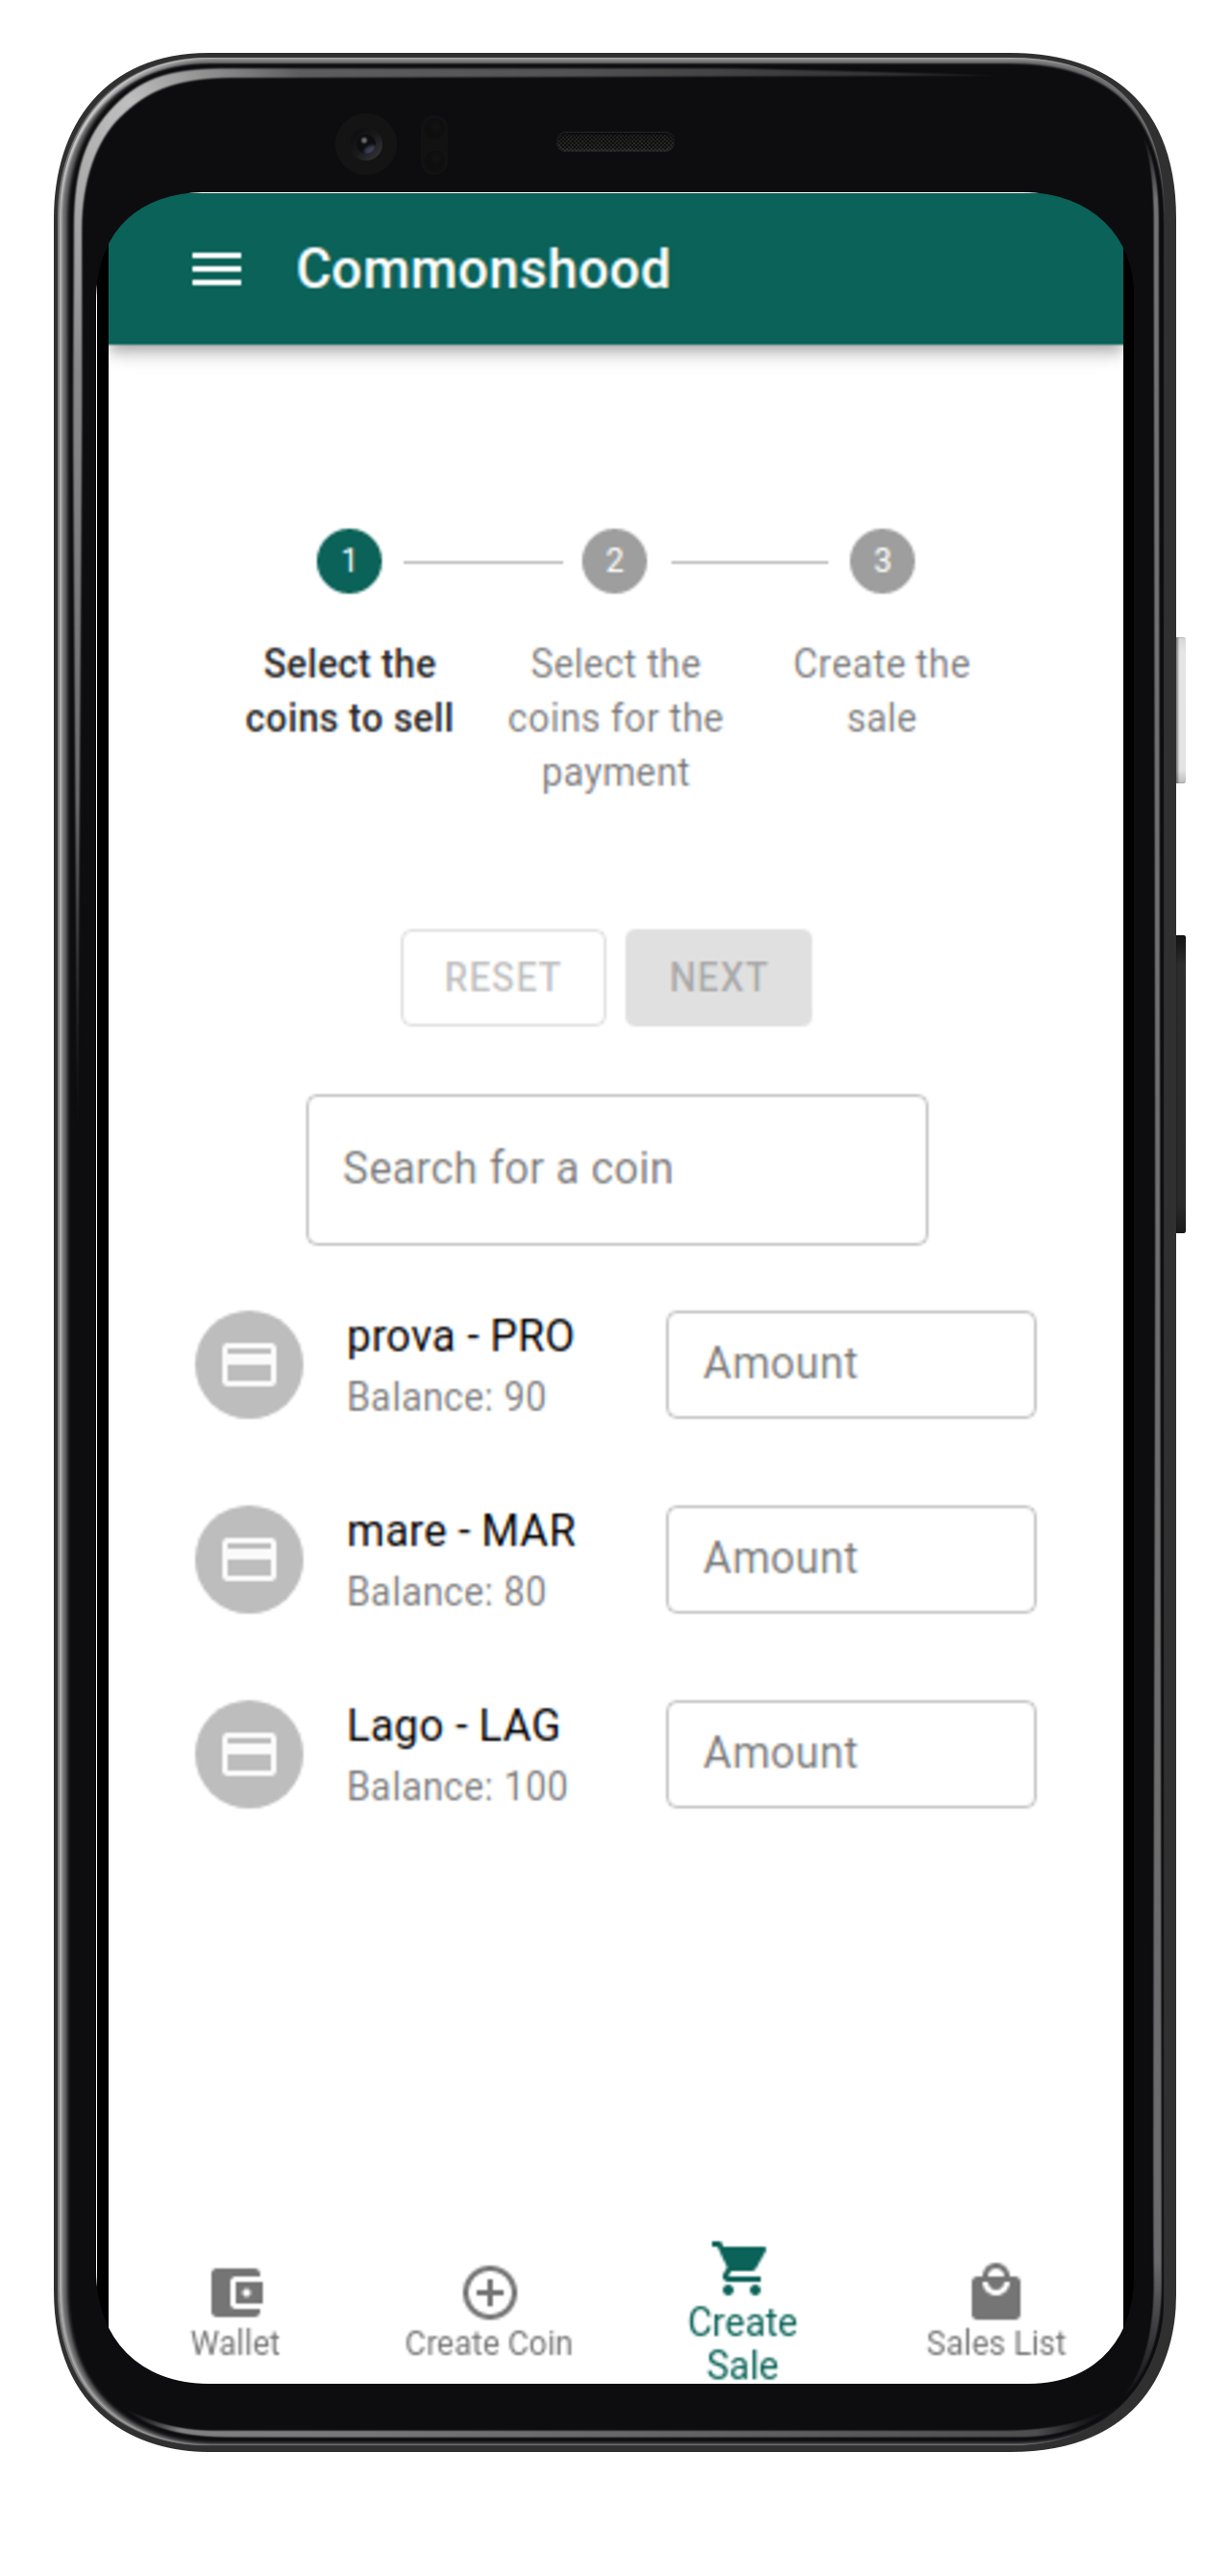
\includegraphics[width=\textwidth]{coinsToSell.png}
          \caption{Pagina per la scelta dei token in vendita}
          \centering
          \label{fig:resume}
        \end{figure}
        La pagina contiene una lista, creata usando il componente \verb|<List>|, ed una barra di ricerca, creata usando il componente \verb|<TextField>|.
        \newline
        Ogni elemento della lista contiene le informazioni di un token posseduto dall'utente e un componente
        \verb|<TextField>|, quest'ultimo permette l'inserimento della quantità desiderata del token da mettere in vendita.
        Gli eventi a cui la pagina reagisce possono essere divisi in tre categorie: caricamento della pagina, inserimento di quantità dei token e
        inserimento di testo nella barra di ricerca.
        \paragraph{Caricamento della pagina}
        Al caricamento della pagina vengono istanziate diverse variabili che gestiscono lo stato della stessa.
        \newpage
        \printbibliography
\end{document}